\begin{frame}
  \frametitle{Introduction and Procedure}
  \begin{columns}
        \column[t]{5cm}
        Many of the new, advanced reactors will use \gls{HALEU} fuel. 
        What are the resource requirements to meet expected \gls{HALEU}
        demand?

        \begin{block}{Procedure}
            Modeled three fuel cycle scenarios using \Cyclus. Simulations 
            model materials from mine to final disposal.
            \begin{itemize}
                \item \textbf{Scenario 1:} Current fleet of \glspl{LWR}
                \item \textbf{Scenario 2:} No growth transition to \gls{USNC} \gls{MMR}
                \item \textbf{Scenario 3:} No growth transition to X-energy Xe-100
            \end{itemize}
 
        \end{block}
        
        \column[t]{5cm}
        \begingroup
        \renewcommand{\arraystretch}{1.5} % Default value: 1
        \begin{table}[t!]
            \tiny
            \caption{Mico-reactor design specifications}
            \label{tab:reactor_summary}
            \begin{tabular}{ p{1.25cm} p{1.25cm} p{1.25cm}}
                \hline
                Design Criteria & \gls{USNC} \gls{MMR}\textsuperscript{TM} & 
                    X-Energy Xe-100\textsuperscript{TM} \\\hline
                
                Reactor Type & Modular HTGR & Modular HTGR \\
                Power Output (MWth) & 15 & 200 \\
                Enrichment (\% $^{235}U$) & 13 & 15.5 \\
                Cycle Length (years) & 20 & Online Refuel\\
                Fuel Form & TRISO Compacts & TRISO Pebbles\\
                Reactor Lifetime & 20 years & 60 years \\
                Coolant & He & He \\
                \hline
            \end{tabular}
        \end{table}   
        \endgroup
  \end{columns}
        
\end{frame}

\begin{frame}
\frametitle{Results}
        \vspace{-0.5cm}
    \begin{columns}
      \column[t]{6cm}
      \begin{figure}[t!]
          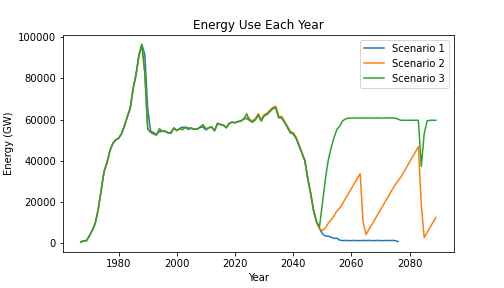
\includegraphics[trim=0 8 0 10,clip,width=\linewidth]{figures/energy_all.png}
            \vspace*{-0.5cm}
          \caption{Total energy output of each scenario.}
          \label{fig:energy}
      \end{figure}
            \vspace*{-0.25cm}
      \begin{figure}[h]
          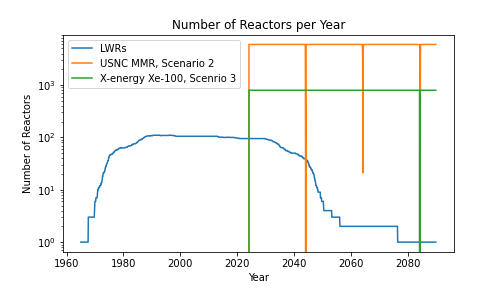
\includegraphics[trim=0 8 0 10,clip,width=\linewidth]{figures/rx_deployment_all.png}
            \vspace*{-0.5cm}
          \caption{Number of each reactor type deployed.}
          \label{fig:ex_deployment}
      \end{figure}
      \column[t]{6cm}
  \begin{figure}[t]
      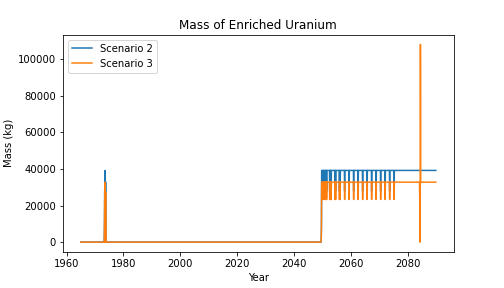
\includegraphics[trim=0 8 0 10,clip,width=\linewidth]{figures/enrichedU_advancedrx.png}
            \vspace*{-0.5cm}
      \caption{Mass of enriched uranium to supply advanced reactors.}
      \label{fig:enrichedU}
  \end{figure}
            \vspace*{-0.5cm}
  \begin{figure}[h]
      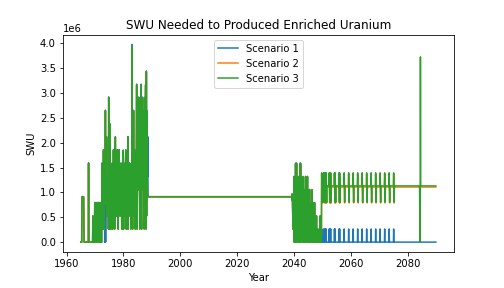
\includegraphics[trim=0 8 0 10,clip,width=\linewidth]{figures/swu_all.png}
            \vspace*{-0.5cm}
      \caption{Total \gls{SWU} capacity required in enrich natural uranium each scenario.}
      \label{fig:swu}
  \end{figure}
  \end{columns}
\end{frame}


\begin{frame}
\frametitle{Conclusions}
    \begin{itemize}
        \item Neither of the transition scenarios (scenarios 2 and 3) meet the desired power level.
        \item Scenario 2 requires a higher mass of \gls{HALEU} than scenario 3.
        \item Scenario 3 requires the most \gls{SWU} capacity.
        \item Scenario 3 involves a large increase in enriched uranium when 
              new reactors are built.
    \end{itemize}

    \begin{block}{Ongoing Work}
        \begin{itemize}
            \item Adjust feed inventory for enrichment facilities.
            \item Ensure simulations are as realistic as possible.
            \item Simulate growth transition scenarios.
            \item Include other reactor types.
        \end{itemize}
    \end{block}
    

\end{frame}
